\documentclass[a4paper]{article}

\usepackage[]{amsmath} 
\usepackage[]{amssymb} 
\usepackage[]{amsthm} 

\usepackage[]{enumerate} 

\usepackage[]{microtype} 
\usepackage[]{mathtools} 
\usepackage[]{minted} 

\usepackage[margin=1.5in]{geometry} 
\usepackage[]{graphicx} 
\graphicspath{{./pictures/}}


\usepackage[]{hyperref} 
\usepackage[capitalize, noabbrev]{cleveref} 

\title{\textsc{Assignment 2 \\ MATINF4170 \\ Spline methods}}
\author{Ivar Haugal{\o}kken Stangeby}

\begin{document}
    \maketitle

    \section*{Exercise 2.2}
    \label{sec:exercise_2_2}
    In this exercise we want to find the individual polynomial pieces of the
    cubic B-splines:
    \begin{enumerate}[i)]
        \item $B[0, 0, 0, 0, 1](x)$;
        \item $B[0, 1, 1, 1, 1](x)$;
        \item $B[0, 1, 1, 1, 2](x)$.
    \end{enumerate}
    Instead of computing these directly, we first show the general claim that
    \begin{equation}
        \notag
        B[a, \overbrace{b, \ldots, b}^p, c](x) = \frac{(x-a)^p}{(b-a)^p}B[a,
        b](x) + \frac{(c-x)^p}{(c-b)^p}B[b, c](x), 
    \end{equation}
    outlined in exercise 2.7 (note that we do allow $a = b$, $b = c$).
    \paragraph{Base case}
    We proceed by induction, and the base case consists of $p = 0$. The right
    hand side then directly evaluates to $B[a, b](x) + B[b, c](x)$, which is
    equal to $B[a, c]$ as the knot intervals are adjacent. 
    
    \paragraph{Induction step} For the inductive
    step, we assume the claim holds for $p = k-1$, and show it must also hold
    for $p = k$. We then have
    \begin{align*}
        B[a, \overbrace{b, \ldots, b}^k, c](x) &= \frac{(x-a)}{(b-a)} B[a,
        \underbrace{\overbrace{b, \ldots, b}^{k-1}, b}_k](x)+
        \frac{(c-x)}{(c-b)}B[\underbrace{b, \overbrace{b, \ldots, b}^{k-1}}_{k},
        c](x),
        \intertext{and applying the induction hypothesis yields}
        &= \frac{(x-a)^k}{(b-a)^k}B[a, b](x) + \frac{(c-x)^k}{(c-b)^k}B[b, c](x).
    \end{align*}
    This closes the induction. It then follows that 
    \begin{enumerate}[i)]
        \item $B[0, 0, 0, 0, 1](x) = (1 - x)^3B[0, 1](x)$;
        \item $B[0, 1, 1, 1, 1](x) = x^3B[0, 1](x)$;
        \item $B[0, 1, 1, 1, 2](x) = x^3B[0, 1](x) + (2 - x)^3B[1, 2](x)$,
    \end{enumerate}
    using the zero-convention. This can be verified by direct computation.
    
    When it comes to smoothness, if we have a knot $t_j$ of multiplicity $m$,
    then the derivatives of the spline $B_{j, p}$ of order $0, 1, \ldots, p -
    m$ are continuous at the knot $t_j$. For the above B-splines, we have knot
    multiplicity of 4, 4 and 3 respectively, hence for $B[0, 0, 0, 0, 1]$ we
    have a discontinuity at $x = 0$ as $p - m = 3 - 4 = -1$. This can also be
    seen by comparing the two limits at 0. By the same token, $B[0, 1, 1, 1,
    1]$ has a discontinuity at $x = 1$. The B-spline $B[0, 1, 1, 1, 2]$ on the
    other hand exhibits $C^0$ continuity at the knot $x = 1$.
    

    \section*{Exercise 2.6}
    
    \subsection*{Induction proof}
    We wish to show the identity
    \begin{equation}
        \label{eq:statement}
        B(t_i \mid t_j, \ldots, t_{j+p+1}) = B(t_j \mid t_i, \ldots, t_{i-1}, t_{i+1}, \ldots, t_{j + i + p})
    \end{equation}
    holds for $i = j, \ldots, j+p+1$. 
    
    \paragraph{Base case:} Note that the B-spline on the right hand
    side is one degree lower than that on the left. Hence, our base case
    consists of $p = 1$. With $p = 1$ we have three cases: $t_i = t_j, t_{j+1}$
    and $t_{j+2}$. In general we have
    \begin{equation}
        \notag
        B(x \mid t_j, t_{j+1}, t_{j+2}) = \frac{x - t_j}{t_{j+1} - t_j} B(x \mid t_j, t_{j+1}) 
                                        + \frac{t_{j+2} - x}{t_{j+2} - t_{j+1}} B(x \mid t_{j+1}, t_{j+2}).
    \end{equation}
    Plugging in $x = t_j$ both terms evaluates to zero, and since $t_j$ is
    outside the interval $[t_{j+1}, t_{j+2})$, the right hand side of
    \cref{eq:statement} also evaluates to zero. By symmetry, the same holds for
    $x = t_{j+2}$. For $x = t_{j+1}$, we get $B(x \mid t_j, t_{j+1}) = 0$,
    while $B(x \mid t_{j+1}, t_{j+2}) = 1$. By definition, the right hand side
    of \cref{eq:statement} also evaluates to 1. This concludes the base case.

    \paragraph{Induction step:}
    For the inductive step, we assume that \cref{eq:statement} holds for degree
    $p - 1$. For degree $p$, the left hand side of \cref{eq:statement} then
    reads:
    {\small
    \begin{align*}
        &B(t_i \mid t_j, \ldots, t_{j+p+1}) = \frac{t_i - t_j}{t_{j+p} - t_j} B(t_i \mid t_j \ldots t_{j+p})
        + \frac{t_{j+p+1} - t_i}{t_{j+p+1} - t_{j+1}} B(t_i \mid t_{j+1} \ldots t_{j+p+1}),
    \intertext{\normalsize which by the induction hypothesis yields}
    &\frac{t_i - t_j}{t_{j+p} - t_j} B(t_i \mid t_j \ldots, t_{i-1}, t_{i+1}, \ldots, t_{j+p}) 
        + \frac{t_{j+p+1} - t_i}{t_{j+p+1} - t_{j+1}}B(t_i \mid t_{j+1}, \ldots, t_{i-1}, t_{i+1}, \ldots, t_{j+p+1}).
    \end{align*}
    }%
    Evaluating the right hand side of \cref{eq:statement} using the recursive
    definition, yields the same result. This closes the induction.
    
    \subsection*{Application}
    
    We use the result proved above to evaluate the second order B-spline $B_{j,
    2}$ at its interior knots, $t_{j+1}$ and $t_{j+2}$. The first interior knot gives
    \begin{equation}
        \notag
        B(t_{j+1} \mid t_j, \ldots, t_{j+3}) = B(t_{j+1} \mid t_j, t_{j+2}, t_{j+3}) 
        = \frac{t_{j+1} - t_j}{t_{j+2} - t_j} \underbrace{B(t_{j+1} \mid t_j, t_{j+2})}_{= 1} = \frac{t_{j+1} - t_j}{t_{j+2} - t_j}.
    \end{equation}
    For the second interior knot, we have
    {\small
    \begin{equation}
        \notag
        B(t_{j+2} \mid t_j, \ldots, t_{j+3}) = B(t_{j+2} \mid t_j, t_{j+1}, t_{j+3}) 
        = \frac{t_{j+3} - t_{j+2}}{t_{j+3} - t_{j+1}} \underbrace{B(t_{j+2} \mid t_{j+1}, t_{j+3})}_{= 1} 
        = \frac{t_{j+3} - t_{j+2}}{t_{j+3} - t_{j+1}}.
    \end{equation}
    }%

    \subsection*{Repeated interior knots}

    Assume now that we all interior knots are equal to some number $z$, i.e.,
    we have knot multiplicity $p$ at interior knots. That is $t_j < z <
    t_{j+p+1}$. By repeated use of the above result, we have that the $j$th
    B-spline can be evaluated as such:
    \begin{equation}
        \notag
        B(z \mid t_j, \underbrace{z, \ldots, z}_{p}, t_{j+p+1}) = B(z \mid t_j, t_{j+p+1}) = 1
    \end{equation}
    as $z$ lies in the interval $[t_j, t_{j+p+1})$. If we instead consider the
    B-splines $B_{i, p}$ where $i \neq j$ evaluated at $z$, then we have two cases:
    \begin{enumerate}[i)]
        \item No equal knots, in which case $B_{i, p}(z) = 0$,
        \item $k \leq p$ equal knots, either at the left or right end of the active knots:
            \begin{align*}
                &B(z \mid t_i, \ldots, t_{i + p - k}, \underbrace{z, \ldots, z}_{k}) = B(z \mid t_i, t_{i + p - k}) = 0
                \intertext{or}
                &B(z \mid \underbrace{z, \ldots, z}_{k}, t_{i+k}, \ldots, t_i + p + 1) = B(z \mid t_{i + k}, \ldots,  t_{i + p + 1}) = 0
            \end{align*}
            by repeated application of above result.
    \end{enumerate}
    
    \section*{Exercise 2.11}
    \label{sec:exercise_2_11}
    
    Given a knot vector $t = \left\{ t_j \right\}_{j=1}^{n+p+1}$ and a real
    number $x \in [t_1, \ldots, t_{n+p+1})$ we often find ourselves needing to
    determine exactly what knot interval the number $x$ lies in, e.g.,
    determine the index $\mu$ such that $t_\mu \leq x < t_{\mu+1}$. There are
    many ways of achieving this, and sometimes one can tailor the procedure to
    current contex in order to achieve better performance. We examine a few
    methods, demonstrated in \textsc{Python}, and for all of these we assume $x
    \in [t_1, \ldots, t_{n+p+1})$. These have yet to be tested in a proper
    setting.

    \paragraph{The Naive Approach}
    \label{par:the_naive_approach}
    This method finds the appropriate index by brute force. It has a linear
    computational complexity.
    \begin{minted}{python}
def IndexNaive(x, knots):
    for i in range(len(knots)-1):
        if knots[i] <= x < knots[i+1]:
            return i
    \end{minted}

    \paragraph{Evaluation approach}
    \label{par:evaluation_approach}
    More often than not, when we repeatedly evaluate B-splines it is because we
    want to compute a set of points on the curve. We can use this, as well as
    the fact that knot sequences are increasing to our advantage. Letting the
    function start searching at the previous index, we significantly reduce the
    number of iterations. 
    \begin{minted}{python}
def IndexEvaluation(x, knots, previous=0):
    for i in range(previous, len(knots-1)):
        if knots[i] <= x < knots[i+1]:
            return i
    \end{minted}
     
    \paragraph{Binary approach}
    \label{par:binary_approach}
    
    Applying a binary search algorithm may also yield a small computational
    advantage. Instead of searching from start of knot vector to end, we start
    in the middle. Using the fact that knots are increasing, we can decide
    whether $x$ lies to the left or to the right of the current knot.

    \begin{minted}{python}
def IndexBinary(x, knots):
    a = 0
    b = len(knots)-1
    while a <= b:
        c = (a + b) // 2
        if knots[c] <= x < knots[c+1]:
            return c
        else:
            if x < knots[c]:
                b = c - 1
            else:
                a = c + 1
    \end{minted}

    \paragraph{Binary evaluation approach}
    \label{par:binary_evaluation_approach}
    
    We could also hope to combine the binary search method with the one using
    the previous index as a starting point, to further narrow down our search
    range. This however, I can only see being more efficient if we evaluate
    points on the curve for a set of increasing parameter values, but that
    are not neccessarily lying in adjacent knot intervals.
    \begin{minted}{python}
def IndexBinaryEvaluation(x, knots, previous=0):
    a = previous
    b = len(knots)-1
    while a <= b:
        c = (a + b) // 2
        if knots[c] <= x < knots[c+1]:
            return c
        else:
            if x < knots[c]:
                b = c - 1
            else:
                a = c + 1
    \end{minted}
    
    \section*{Exercise 2.12}
    
    In this exercise we want to implement the algorithm for evaluation non-zero
    B-splines for a given $x$. Given an $x$, we use the binary search algorithm
    outlined above for finding the corresponding index $\mu$ such that $x \in
    [t_\mu, t_{\mu+1})$. The code was implemented in \mathsc{Python}, and can
    be seen in \cref{lst:bsplines}. The algorithm was used to compute and
    visualize the four non-zero B-splines of order $3$ on the uniform knot
    vector $t = \left\{j\right\}_{j=0}^9$.
    \begin{listing}
        \begin{minted}{python} 
def BSplineEvaluation(x, p, knots):
    """
    Evaluate the p+1 active B-splines at the point x.
    Given x, find the index mu such that knots[mu] <= x < knots[mu+1].
    We only need the knots knots[mu - p + 1] to knots[mu + p].
    """ 
    knots = np.array(knots, dtype=np.float64)
    mu = index(x, knots)
    b = 1
    for k in range(1, p+1):
        # extract relevant knots, using array-views to save memory
        t1 = knots[mu - k + 1 : mu+1]
        t2 = knots[mu+1 : mu + k+1]
        # append 0 to end of first term, and insert 0 to start of first term
        omega = (x - t1) / (t2 - t1)
        b = np.append((1 - omega)*b, 0)  + np.insert((omega * b), 0, 0)
    return b
        \end{minted}
        \caption{Given $x$, a degree $p$, and a knot vector, returns the vector
        $b$ consisting of the $p+1$ non-zero B-splines of order $p$ evaluated
    at $x$. Makes use of the \texttt{numpy}-vector operations.}
    \label{lst:bsplines}
    \end{listing}
    
    \begin{figure}[htpb]
        \centering
        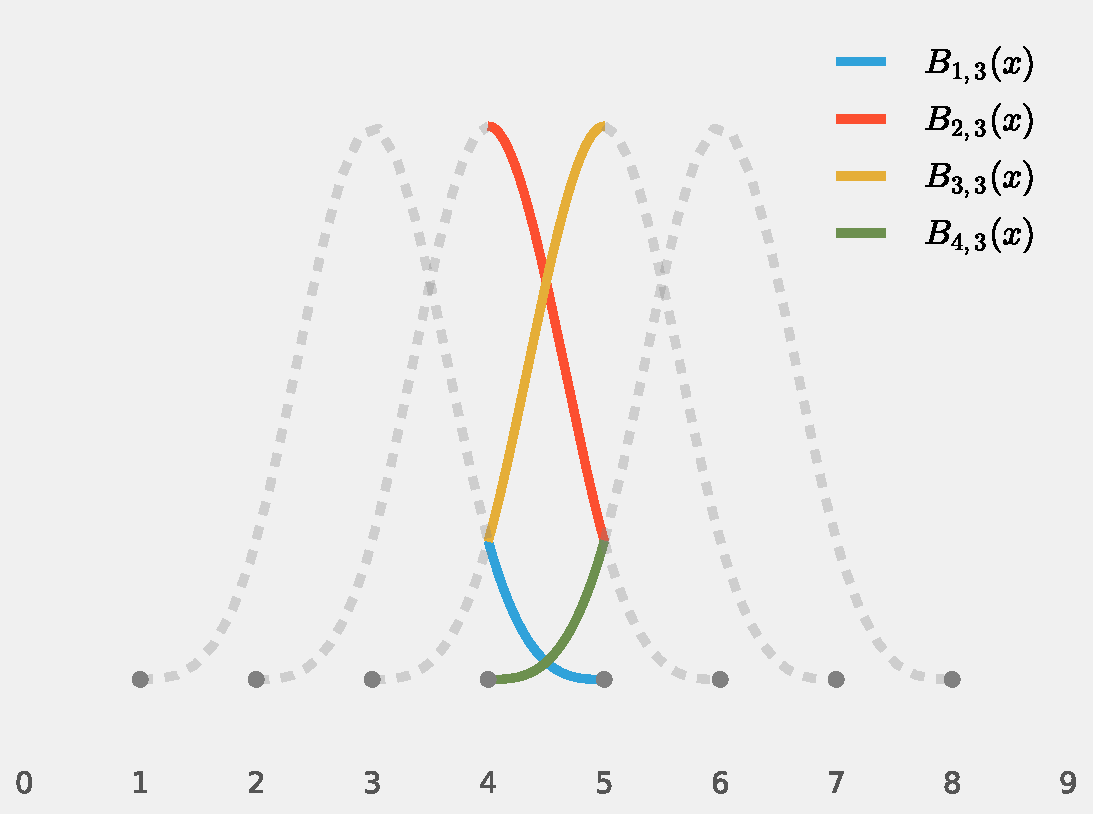
\includegraphics[width=0.8\linewidth]{active_b_splines.pdf}
        \caption{The four active B-splines of order 3 on a uniform knot.}
        \label{fig:active_b_splines.}
    \end{figure}
\end{document}
